\documentclass[tikz,border=4pt]{standalone}
% Estilo común de los diagramas de bloques (se usa con \input en cada standalone)
\usepackage[defaultsans,scale=0.92]{lato}
\usepackage{libertinust1math}
\usepackage{xcolor,amsmath}
\usepackage{tikz}
\usetikzlibrary{positioning,arrows.meta,calc,shapes.geometric}
\usepackage{../../notacion}
\definecolor{ctrlazul}{HTML}{1E5AA8}\definecolor{ctrlnoche}{HTML}{14213D}
\definecolor{ctrlcoral}{HTML}{D1495B}\definecolor{ctrlverde}{HTML}{2A9D8F}
\definecolor{ctrlambar}{HTML}{E09F3E}\definecolor{ctrlgris}{HTML}{5C677D}
\definecolor{ctrlvioleta}{HTML}{6C4AB6}\definecolor{ctrlteal}{HTML}{0F7173}
\tikzset{
  >={Stealth[length=2.4mm]}, every node/.style={font=\small},
  bloque/.style={draw=ctrlnoche,fill=ctrlazul!7,thick,rounded corners=1.5pt,minimum height=9mm,minimum width=13mm,inner sep=4pt},
  suma/.style={draw=ctrlnoche,thick,circle,inner sep=0pt,minimum size=6mm},
  senal/.style={->,thick,draw=ctrlnoche},
  rot/.style={font=\footnotesize,text=ctrlgris},
}

\begin{document}
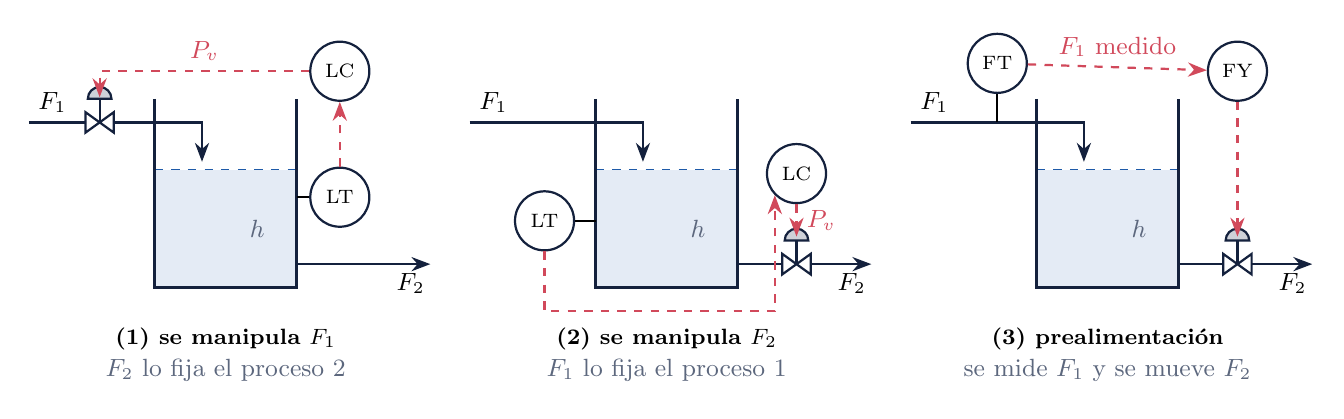
\begin{tikzpicture}[font=\footnotesize,
  valvula/.pic={\draw[thick,ctrlnoche,fill=white] (-0.18,-0.13)--(0.18,0.13)--(0.18,-0.13)--(-0.18,0.13)--cycle; \draw[thick,ctrlnoche] (0,0)--(0,0.3); \draw[thick,ctrlnoche,fill=ctrlgris!30] (-0.15,0.3) arc (180:0:0.15)--cycle;},
  inst/.style={circle,draw=ctrlnoche,thick,fill=white,minimum size=7.5mm,inner sep=0pt,font=\scriptsize},
  inf/.style={dashed,thick,draw=ctrlcoral,->}]
  \newcommand{\tanque}{%
    \fill[ctrlazul!12] (0,0) rectangle (1.8,1.5); \draw[ctrlazul,dashed] (0,1.5)--(1.8,1.5);
    \draw[very thick,ctrlnoche] (0,2.4)--(0,0)--(1.8,0)--(1.8,2.4);
    \draw[thick,ctrlnoche] (-1.6,2.1)--(0.6,2.1)--(0.6,1.75); \draw[senal] (0.6,1.85)--(0.6,1.6);
    \draw[thick,ctrlnoche] (1.8,0.3)--(3.4,0.3); \draw[senal] (3.0,0.3)--(3.5,0.3);
    \node[above] at (-1.3,2.1) {$F_1$}; \node[below] at (3.25,0.3) {$F_2$};
    \node[ctrlgris] at (1.3,0.75) {$h$};}
  % escenario 1
  \begin{scope}
    \tanque \pic at (-0.7,2.1) {valvula};
    \node[inst] (LT) at (2.35,1.15) {LT}; \draw[thick] (1.8,1.15)--(LT);
    \node[inst] (LC) at (2.35,2.75) {LC};
    \draw[inf] (LT)--(LC); \draw[inf] (LC)-|node[pos=0.25,above,text=ctrlcoral]{$P_v$}(-0.7,2.42);
    \node[font=\footnotesize\bfseries] at (0.9,-0.65) {(1) se manipula $F_1$};
    \node[text=ctrlgris] at (0.9,-1.05) {$F_2$ lo fija el proceso 2};
  \end{scope}
  % escenario 2
  \begin{scope}[xshift=5.6cm]
    \tanque \pic at (2.55,0.3) {valvula};
    \node[inst] (LT) at (-0.65,0.85) {LT}; \draw[thick] (0,0.85)--(LT);
    \node[inst] (LC) at (2.55,1.45) {LC};
    \draw[inf] (LT)--(-0.65,-0.3)-|(LC.south west); \draw[inf] (LC)--node[right,text=ctrlcoral]{$P_v$}(2.55,0.65);
    \node[font=\footnotesize\bfseries] at (0.9,-0.65) {(2) se manipula $F_2$};
    \node[text=ctrlgris] at (0.9,-1.05) {$F_1$ lo fija el proceso 1};
  \end{scope}
  % escenario 3
  \begin{scope}[xshift=11.2cm]
    \tanque \pic at (2.55,0.3) {valvula};
    \node[inst] (FT) at (-0.5,2.85) {FT}; \draw[thick] (-0.5,2.1)--(FT);
    \node[inst] (FF) at (2.55,2.75) {FY};
    \draw[inf] (FT)--node[above,text=ctrlcoral]{$F_1$ medido}(FF); \draw[inf] (FF)--(2.55,0.65);
    \node[font=\footnotesize\bfseries] at (0.9,-0.65) {(3) prealimentación};
    \node[text=ctrlgris] at (0.9,-1.05) {se mide $F_1$ y se mueve $F_2$};
  \end{scope}
\end{tikzpicture}
\end{document}
